%%%%%%%%%%%%%%%%%%%%%%%%%%%%%%%%%%%%%%%%%%
%%%%%%%%%%%%%                 %%%%%%%%%%%%
%%%%%%%%%%%%%    EXERCISE 1   %%%%%%%%%%%%
%%%%%%%%%%%%%                 %%%%%%%%%%%%
%%%%%%%%%%%%%%%%%%%%%%%%%%%%%%%%%%%%%%%%%%
\begin{exercise}[]{In this problem we consider sending real-time voice from Host $A$ to Host $B$ over a packet-switched network (VoIP). Host A converts analog voice to a digital $64 \mathrm{kbps}$ bit stream on the fly. Host A then groups the bits into 56 -byte packets. There is one link between Host A and B; its transmission rate is 2 Mbps and its propagation delay is 10 msec. As soon as Host A gathers a packet, it sends it to Host $\mathrm{B}$. As soon as Host $\mathrm{B}$ receives an entire packet, it converts the packet's bits to an analog signal. How much time elapses from the time a bit is created (from the original analog signal at Host A) until the bit is decoded (as part of the analog signal at Host B)? (10 points)}
  \begin{solution}
  \par{~}
  Time for creating a packet $\frac{56 \times 8}{64 \times 10^3} = 7 ms$

  Transmission Time $\frac{56 \times 8}{2 \time 10^6} = 224 \mu s$

  Propagation Delay 10 ms.

  Total time $= 7 + 0.224 + 10 = 17.224 ms$
  \end{solution}
  \label{ex1}
\end{exercise}



%%%%%%%%%%%%%%%%%%%%%%%%%%%%%%%%%%%%%%%%%%
%%%%%%%%%%%%%                 %%%%%%%%%%%%
%%%%%%%%%%%%%    EXERCISE 2   %%%%%%%%%%%%
%%%%%%%%%%%%%                 %%%%%%%%%%%%
%%%%%%%%%%%%%%%%%%%%%%%%%%%%%%%%%%%%%%%%%%
\begin{exercise}[]{Suppose users share a 3 Mbps link. Also suppose each user requires $150 \mathrm{kbps}$ when transmitting, but each user transmits only 10 percent of the time. (See the discussion of statistical multiplexing in Section 1.3.) ( 20 points)
    \begin{enumerate}
        \item When circuit switching is used, how many users can be supported? (5 points)
        \item For the remainder of this problem, suppose packet switching is used. Find the probability that a given user is transmitting. (5 points)
        \item Suppose there are 120 users. Find the probability that at any given time, exactly n users are transmitting simultaneously. (Hint: Use the binomial distribution.) (5 points)
        \item Find the probability that there are 21 or more users transmitting simultaneously. (5 points)
    \end{enumerate}
    }
  \begin{solution}
  \par{~}
  \begin{enumerate}
    \item $3M/150K = 20$ users are supported.
    \item Probability is $\frac{1}{10}$, since we know each user will be using 10\% of the transmission time.
    \item Probability is $C_{120}^{n} \left(\frac{1}{10}\right)^n \left(\frac{9}{10}\right)^{(120-n)}$
    \item Probability is $\sum_{n=21}^{120}C_{120}^{n} \left(\frac{1}{10}\right)^n \left(\frac{9}{10}\right)^{(120-n)} = 0.007941$
  \end{enumerate}
  \end{solution}
  \label{ex2}
\end{exercise}

%%%%%%%%%%%%%%%%%%%%%%%%%%%%%%%%%%%%%%%%%%
%%%%%%%%%%%%%                 %%%%%%%%%%%%
%%%%%%%%%%%%%    EXERCISE 3   %%%%%%%%%%%%
%%%%%%%%%%%%%                 %%%%%%%%%%%%
%%%%%%%%%%%%%%%%%%%%%%%%%%%%%%%%%%%%%%%%%%
\begin{exercise}[]{Suppose two hosts, $A$ and $B,$ are separated by 20,000 kilometers and are connected by a direct link of $R=2 M b p s .$ Suppose the propagation speed over the link is $2.5 \times 10^{8}$ meters/sec. (30 points)

    \begin{enumerate}
        \item Calculate the bandwidth-delay product, $R \times d_{\text {drop }}$ ( 5 points)
        \item Consider sending a file of 800,000 bits from Host A to Host B. Suppose the file is sent continuously as one large message. What is the maximum number of bits that will be in the link at any given time? ( 5 points)
        \item Provide an interpretation of the bandwidth-delay product. (5 points)
        \item What is the width (in meters) of a bit in the link? Is it longer than a football field? (5 points)
        \item Derive a general expression for the width of a bit in terms of the propagation speeds, the transmission rate $R$, and the length of the link $m$. (5 points)
    \end{enumerate}}
  \begin{solution}
  \par{~}
  \begin{enumerate}
    \item $d_{prop} = \frac{20,000 \times 10^3}{2.5 \times 10^8} = 0.08s$, $R\times d_{prop} = 0.16 Mb$
    \item $d_{trans} = \frac{800 kb}{2Mbps} = 0.4s > 0.08s$. There exists a moment where the whole link has bits transmitting. The maximum number of bits is $0.16 Mb$.
    \item The bandwidth-delay product on a link can be interpreted as the maximum number of bits that will be in the link.
    \item $\frac{20,000 Km}{0.16 Mb} = 125m$. Longer than a football field.
    \item The general expression for the width of a bit $l$ is
    \begin{equation}
      l = \frac{S}{R \times d_{prop}} = \frac{S}{\frac{R \times S}{v}} = \frac{v}{R}
    \end{equation}
    where $R$ is the transmission rate and $v$ is propagation speed.
  \end{enumerate}
  \end{solution}
  \label{ex3}
\end{exercise}



%%%%%%%%%%%%%%%%%%%%%%%%%%%%%%%%%%%%%%%%%%
%%%%%%%%%%%%%                 %%%%%%%%%%%%
%%%%%%%%%%%%%    EXERCISE 4   %%%%%%%%%%%%
%%%%%%%%%%%%%                 %%%%%%%%%%%%
%%%%%%%%%%%%%%%%%%%%%%%%%%%%%%%%%%%%%%%%%%
\begin{exercise}[]{In modern packet-switched networks, the source host segments long, application- layer messages (for example, an image or a music file) into packets and sends the packets into the network. The receiver then reassembles the packets back into the original message. We refer to this process as message segmentation. Figure 1 illustrates the end-to-end of a message with and without message segmentation. Consider a message that is $8 \times 10^6$ bits long that is to be sent from source to destination in Figure \ref{fig1}. Suppose each link in the figure is 2 Mbps. Ignore propagation, queuing, and processing delays. (20 points)
    
    \begin{figure}[hb]
      \begin{center}
      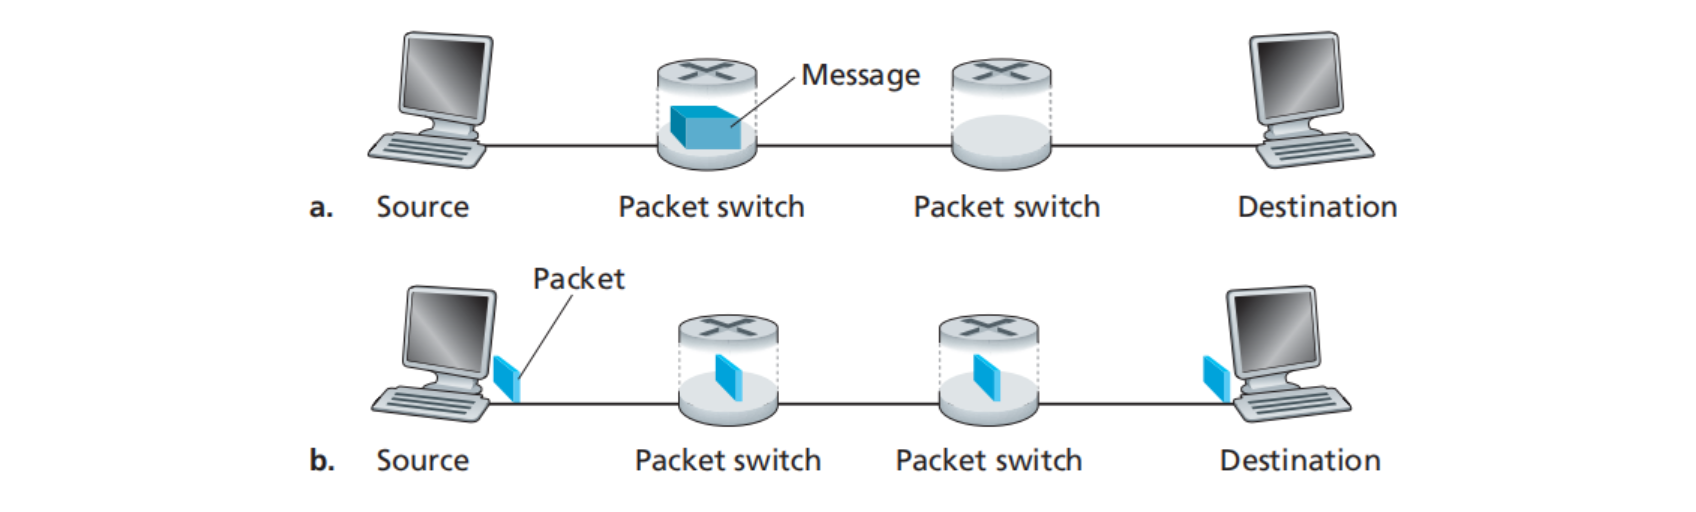
\includegraphics[width=12cm]{img/ass1/fig1}
      \caption{End-to-end message transport: (a) without message segmentation; (b) with message segmentation}
      \label{fig1}
      \end{center}
    \end{figure}

    \begin{enumerate}
        \item Consider sending the message from source to destination without message segmentation. How long does it take to move the message from the source host to the first packet switch? Keeping in mind that each switch uses store-and-forward packet switching, what is the total time to move the message from source host to destination host? (5 points)
        \item  Now suppose that the message is segmented into 4,000 packets, with each packet being 2,000 bits long. How long does it take to move the first packet from source host to the first switch? When the first packet is being sent from the first switch to the second switch, the second packet is being sent from the source host to the first switch. At what time will the second packet be fully received at the first switch? (5 points)
        \item How long does it take to move the file from source host to destination host when message segmentation is used? Compare this result with your answer in part (a) and comment. (5 points)
        \item Discuss the drawbacks of message segmentation. (5 points)
    \end{enumerate}
    }
  \begin{solution}
  \par{~}
  \begin{enumerate}
    \item Each hop takes $\frac{8 \times 10^6}{2\times 10^6} = 4s$. Store and forward takes $3 \times 4 = 12s$
    \item It takes $\frac{2000}{2\times 10^6} = 1ms$ to transmit the first packet to the first switch. At $2ms$ the second packet will fully be received at the first switch.
    \item Time for packet 1 to reach destination is $3ms$, After this, every $1ms$ a packet will arrive. Totally, it will take $3 + 3999 \times 1 = 4.002s$. It can be seen that with message segmentation, the delay is reduced to $1/3$ of the original.
    \item Drawbacks: more complicated protocols need to be designed in order to ensure the reassembling works well and all the data are transmitted. It will also require the host to be able to meet certain condiitons in order to reassemble the data.
  \end{enumerate}
  \end{solution}
  \label{ex4}
\end{exercise}


%%%%%%%%%%%%%%%%%%%%%%%%%%%%%%%%%%%%%%%%%%
%%%%%%%%%%%%%                 %%%%%%%%%%%%
%%%%%%%%%%%%%    EXERCISE 5   %%%%%%%%%%%%
%%%%%%%%%%%%%                 %%%%%%%%%%%%
%%%%%%%%%%%%%%%%%%%%%%%%%%%%%%%%%%%%%%%%%%
\begin{exercise}[]{For a $4 \mathrm{kHz}$ voice channel with signal-to-noise ratio $30 \mathrm{~dB} .$ Is it possible to provide 56kbps data rate service? (5 points)}
  \begin{solution}
  \par{~} By Shannon's Theorem, the upper bound of the channel capacity is
  \begin{equation}
     C = B \times \log_2 (1 + SNR) = 4 KHz \times \log_2 (1 + 10^{(30/10)}) = 39.868 Kbps \le 56 Kbps
  \end{equation}
  The channel can't provide 56kbps data rate service.
  \end{solution}
  \label{ex5}
\end{exercise}


%%%%%%%%%%%%%%%%%%%%%%%%%%%%%%%%%%%%%%%%%%
%%%%%%%%%%%%%                 %%%%%%%%%%%%
%%%%%%%%%%%%%    EXERCISE 6   %%%%%%%%%%%%
%%%%%%%%%%%%%                 %%%%%%%%%%%%
%%%%%%%%%%%%%%%%%%%%%%%%%%%%%%%%%%%%%%%%%%
\begin{exercise}[]{Compare the delay in sending an $x$ -bit message over a $k$ -hop path in a circuitswitched network and in a (lightly loaded) packet-switched network. The circuit setup time is $s$ sec, the propagation delay is $d$ sec per hop, the packet size is $p$ bits $(p<x),$ and the data rate is $b$ bps. Under what conditions does the packet network have a lower delay? (Ignore queuing delay, and processing delay.) (15 points)
    
    Please note: for multiple packets in packet-switched network, the transmission is pipelined,
    i.e., more than one packets can be transmitted in sequence at the same time. So we have $D_{e n d-t o-e n d} \neq \sum d_{e n d-t o-e n d-i}(i$ is the packet No.)}
  \begin{solution}
  \par{~}
  For Circuit Switching, a link from source to destination is required to setup. Then all bits are transmitted and propagated. $Delay = s + x/b + kd$

  For Packet Switching, consider the first packet. It does not require a setup, but the store-and-forward strategy requires $(k - 1)p/b$ transmission delay. With pipelined packet-switching, the delay of other packets can be discarded. Total Delay $= x/b + (k - 1)p/b + kd$.

  Packet Switching is better than Circuit Switching if $s > (k-1)p/b$
  \end{solution}
  \label{ex6}
\end{exercise}